\documentclass{article}
\usepackage{pgf}
\usepackage{tikz}
\usepackage{amsmath, amssymb}
\usetikzlibrary{arrows.meta}
\usepackage[utf8]{inputenc}
\begin{document}
    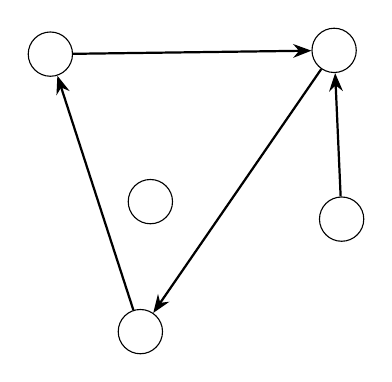
\begin{tikzpicture}[scale=0.6,auto]
        \tikzset{>=Stealth}
        \tikzstyle{every path}=[->,thick]
        \tikzstyle{every node}=[circle,fill=white,draw=black,text=black,thin,minimum size=16pt,inner sep=1.5pt]

        \node (n1) at (1.8310416666666671cm,-1.2754166666666666cm) {};
        \node (n2) at (7.837083333333334cm,-1.196041666666667cm) {};
        \node (n3) at (3.736041666666667cm,-7.149166666666668cm) {};
        \node (n4) at (7.995833333333334cm,-4.767916666666667cm) {};
        \node (n5) at (3.947708333333334cm,-4.397500000000001cm) {};

        \draw (n2) to (n3);
        \draw (n4) to (n2);
        \draw (n3) to (n1);
        \draw (n1) to (n2);
    \end{tikzpicture}
\end{document}
